% !TeX spellcheck = it_IT

%Controllare anche RFC per studiare
\section{Ad Hoc Distance Vector Routing Protocol AODV}

Ambito WLAN. Si tratta di un \textbf{protocollo di routing}: ha il compito di \textbf{creare e riempire le tabelle di instradamento}. Pensato per una \textbf{rete senza infrastrutture} in cui ogni nodo è anche un router (può fare instradamento). I cammini possono essere multi-hop. I nodi vicini sono quelli nel raggio radio, di conseguenza nodi e vicinati possono variare.\\
I percorsi non vengono creati in modo proattivo: quando serve mandare qualcosa viene richiesto il percorso.\\

Gli \textbf{obiettivi} principali del protocollo sono:
\begin{itemize}
	\item Gestione dinamica della rete ad hoc, ogni nodo può operare secondo protocollo
	\item Auto inizializzante, non sono necessarie rotte preconfigurate; l'inizializzazione deve essere fatta in automatico e periodicamente (per "colpa" della dinamicità della rete)
	\item Loop-free (eliminando il problema del counting to infinity)
	\item Ottenimento di una rotta per una nuova destinazione in tempi rapidi
	\item Risposta rapida alla rottura dei link e al cambio di topologia
\end{itemize}

Le \textbf{funzionalità} che offre sono:
\begin{itemize}
	\item Scoprire e costruire i percorsi per le nuove destinazioni
	\item Mantenere i percorsi in modalità soft-state; ogni percorso ha una durata, se non "rinfrescata" la entry scade e può essere cancellata (eventually)
	\item Riconoscimento errori e cancellazione di percorsi; monitoraggio dell'attività locale e propagazione delle informazioni
\end{itemize}

Si tratta di un protocollo a livello di applicazione (usa UPD 654) che permette di creare tabelle di routing a livello di rete. Ogni nodo è responsabile delle proprie entry, il protocollo è completamente distribuito.\\

\newpage

I dati vengono inviati tra originator e destinazione tramite percorsi simmetrici, non ci sono percorsi indipendenti.
\begin{center}
	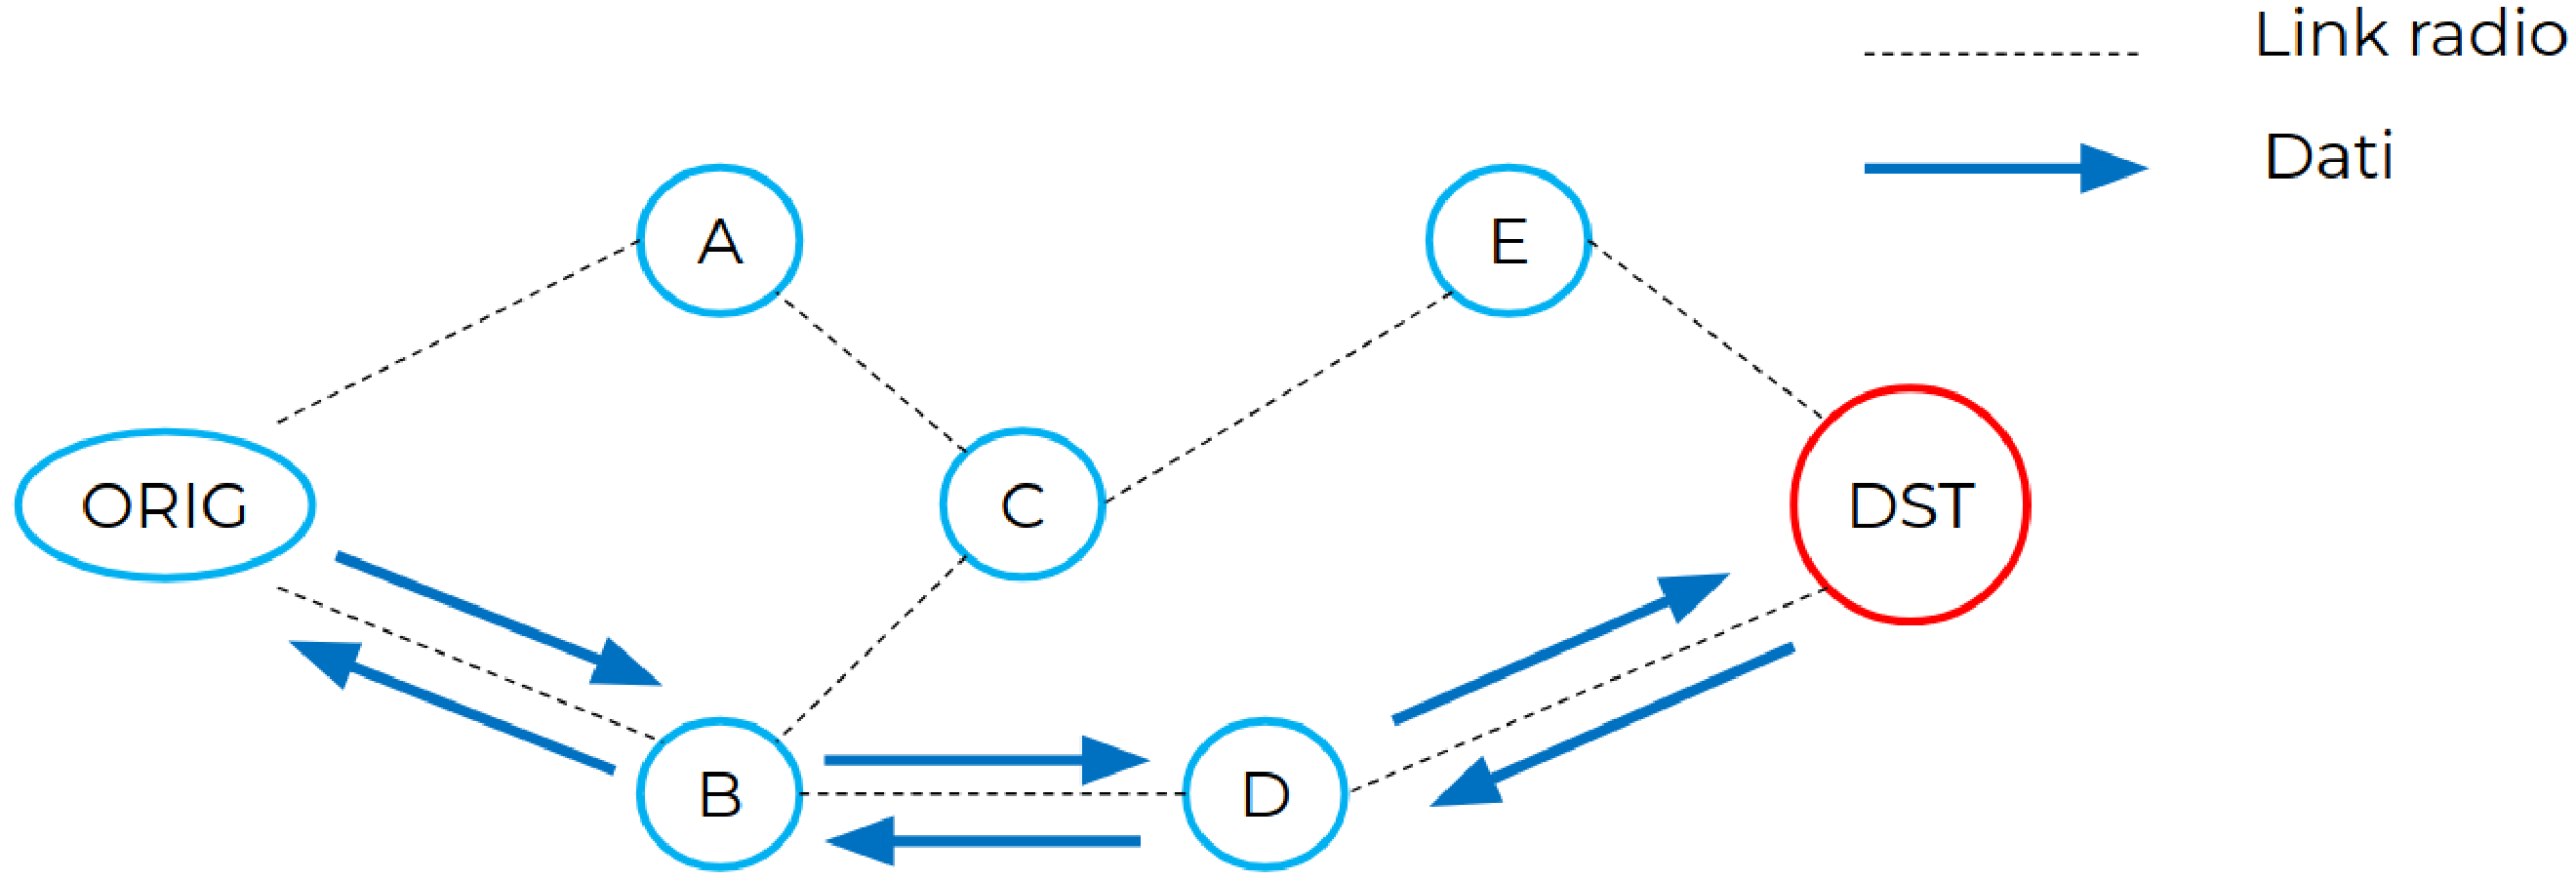
\includegraphics[width=0.9\linewidth]{img/aodv/path1}
\end{center}

\paragraph{Route Request:} I percorsi vengono costruiti tramite \textbf{Route Request RREQ}, sono pacchetti di controllo che permettono di chiedere la costruzione di un percorso verso la destinazione. Non sapendo niente, i messaggi RREQ vengono inviati in broadcast "controllato" (senza loop, il broadcast è fatto a livello IP, con l'indirizzo IP di broadcast). Ogni nodo inoltra RREQ e tiene traccia della provenienza.\\

\paragraph{Route Reply:} La destinazione richiesta in una RREQ risponde in unicast con un messaggio \textbf{Route Reply RREP}.
\begin{center}
	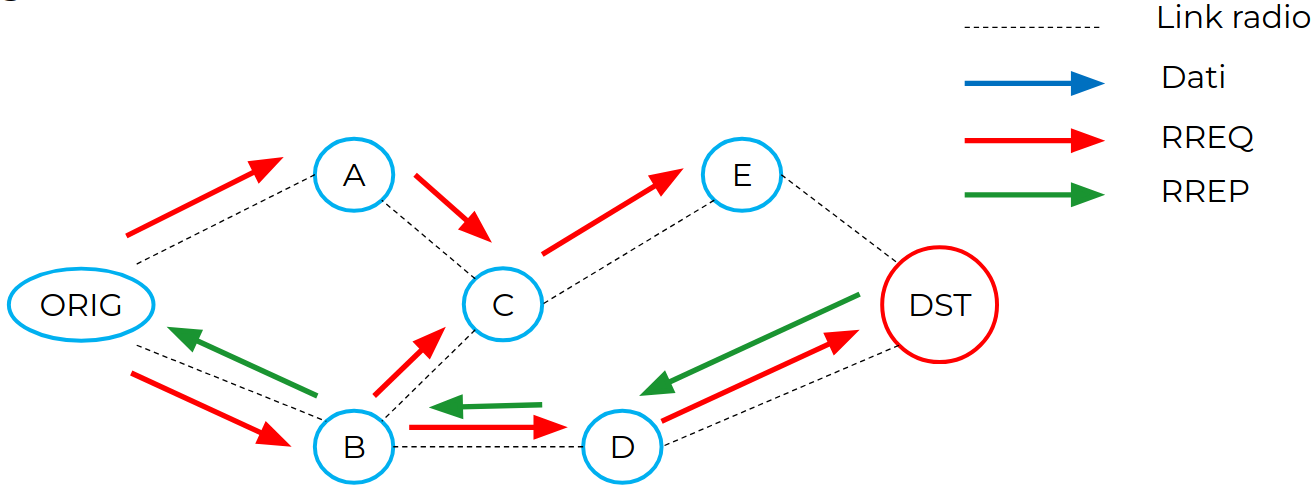
\includegraphics[width=0.9\linewidth]{img/aodv/path2}
\end{center}

La destinazione manda la risposta RREP solo alla prima RREQ (con lo stesso identificatore) ricevuta, in modo da evitare risposte duplicate e trovando (circa) il percorso più breve, dato che risponderà solo al messaggio che ci ha impiegato meno tempo (il primo arrivato).\\

Anche un nodo intermedio può fornire la risposta (inviare il RREP), se conosce l'informazione (sa come arrivare a destinazione) ed è abbastanza "fresca" (lo ha saputo di recente).\\

\paragraph{Route Error:} Un altro messaggio di controllo è \textbf{Route Error RERR}, usato nel caso un link si rompe, per qualsiasi motivo. Il nodo lo invia a tutti i vicini che sa utilizzano quel link per arrivare ad una qualche destinazione.\\

Lo stack è:

\begin{center}
	\renewcommand{\arraystretch}{1.4}
	\begin{tabular}{>{\centering\arraybackslash}m{4cm} | >{\centering\arraybackslash}m{3.5cm} | >{\centering\arraybackslash}m{3.5cm} |}
		\cline{2-3}
		& Messaggi Dati & RREQ/RREP/RERR \\
		\hline
		Livello applicazione & Protocollo\newline applicazione & AODV \\
		\hline
		Livello Trasporto & Trasporto \newline UPD/TCP/\dots & UPD Porta 654 \\
		\hline 
		Livello Rete & \multicolumn{2}{c |}{IP} \\
		\hline
		Livello data link (LL) & \multicolumn{2}{c |}{Ethernet (802.3)/WiFi(802.11)/802.15.4/\dots} \\
		\hline
		Livello fisico (PHY) & \multicolumn{2}{c |}{Ethernet (802.3)/WiFi(802.11)/802.15.4/\dots} \\
		\hline
	\end{tabular}
\end{center}
Quindi i messaggi possono essere dati "normali" tramite TCP oppure i messaggi di controllo AODV. Il livello di rete è IP, mentre i livelli di data link e fisico possono essere uno qualsiasi degli standard IEEE previsti.\\

\subsection{Tabelle di Routing}

Ogni nodo mantiene una tabella delle destinazioni conosciute e l'indicazione del prossimo hop lungo il percorso. Ogni entry in una tabella contiene:
\begin{itemize}
	\item IP destinazione
	\item Sequence number della destinazione
	\item Flag di validità del sequence number della destinazione; permette di disabilitare/abilitare temporaneamente un percorso
	\item Stato del percorso (valido, invalido e altri)
	\item Interfaccia di rete
	\item Hop count, numero di hop per arrivare alla destinazione, ovvero il costo
	\item Lista dei precursori, quali sono i vicini che utilizzano "me" (il nodo) per arrivare a destinazione
	\item Lifetime della entry, ovvero il tempo di scadenza
\end{itemize}

\paragraph{Sequence Number SN:} Tutto cambia in questa rete, quindi ogni entry della tabella possiede un SN che codifica informazioni circa "\textit{la freschezza}" della entry stessa. Il SN è un valore per ogni nodo, ogni possibile destinazione (nodo) ha il proprio e viene modificato esclusivamente dal nodo stesso. \\

Il SN viene incrementato dal nodo in 2 casi: 
\begin{enumerate}
	\item Quando un nodo inizia una ricerca di percorso (RREQ), viene incrementato di 1, previene conflitti con i percorsi inversi stabiliti da una precedente RREQ
	\item Quando un nodo risponde (ovvero il nodo è la destinazione) ad una richiesta di percorso (manda RREP); si aumenta di 1 (solo in alcuni casi in realtà)
\end{enumerate}

Gli altri nodi possono aggiornare il sequence number di una entry in tabella se: 
\begin{itemize}
	\item Il nodo stesso offre un nuovo percorso per se stesso (aggiorna la propria entry nella sua tabella di routing)
	\item Il nodo riceve informazioni più aggiornate per un destinazione
	\item Il percorso verso quella destinazione è scaduto/interrotto
\end{itemize}

Il SN viene confrontato per capire \textit{chi ha l'informazione più aggiornata} per la destinazione. L'incremento viene fatto come se fosse unsigned, il confronto come signed (per gestire overflow).\\

\newpage

\subsection{RREQ}

\paragraph{Formato:} Il formato di una RREQ è 
\begin{verbatim}
	 0                   1                   2                   1
	 0 1 2 3 4 5 6 7 8 9 0 1 2 3 4 5 6 7 8 9 0 1 2 3 4 5 6 7 8 9 0 1
	+-+-+-+-+-+-+-+-+-+-+-+-+-+-+-+-+-+-+-+-+-+-+-+-+-+-+-+-+-+-+-+-+
	|     Type      |J|R|G|D|U|   Reserved          |   Hop Count   |
	+-+-+-+-+-+-+-+-+-+-+-+-+-+-+-+-+-+-+-+-+-+-+-+-+-+-+-+-+-+-+-+-+
	|                            RREQ ID                            |
	+-+-+-+-+-+-+-+-+-+-+-+-+-+-+-+-+-+-+-+-+-+-+-+-+-+-+-+-+-+-+-+-+
	|                    Destination IP Address                     |
	+-+-+-+-+-+-+-+-+-+-+-+-+-+-+-+-+-+-+-+-+-+-+-+-+-+-+-+-+-+-+-+-+
	|                  Destination Sequence Number                  |
	+-+-+-+-+-+-+-+-+-+-+-+-+-+-+-+-+-+-+-+-+-+-+-+-+-+-+-+-+-+-+-+-+
	|                     Originator IP Address                     |
	+-+-+-+-+-+-+-+-+-+-+-+-+-+-+-+-+-+-+-+-+-+-+-+-+-+-+-+-+-+-+-+-+
	|                  Originator Sequence Number                   |
	+-+-+-+-+-+-+-+-+-+-+-+-+-+-+-+-+-+-+-+-+-+-+-+-+-+-+-+-+-+-+-+-+
\end{verbatim}

Il \textbf{tipo} è 1, rappresenta il tipo di pacchetto di controllo inviato (RREQ in questo caso).\\

Le \textbf{flag} sono: 
\begin{itemize}
	\item \textbf{\texttt{D}}: Destination Only, solo la destinazione può rispondere, niente nodi intermedi
	\item \textbf{\texttt{U}}: Unknown SN, l'origine non conosce SN della destinazione
	\item \textbf{\texttt{G}}: (Gratuitous) RREP, un nodo intermedio, oltre a rispondere all'origine, deve informare la destinazione della creazione di un percorso (reverse) con l'origine
\end{itemize}

L'\textbf{hop count} viene incrementato di 1 ogni volta che viene inoltrata la RREQ, serve a tenere traccia del "costo" del percorso, in realtà la destinazione vuole rispondere alla RREQ con hop count minore.\\

Il \textbf{RREQ ID} è l'identificativo della richiesta, generato dall'origine e mai modificato, serve a riconoscere la richiesta e le sue copie come un'unica richiesta all'interno della rete.\\

\newpage

Il \textbf{Destination IP Address} è l'indirizzo della destinazione ed il SN indicato è l'ultimo conosciuto (o nessuno nel caso il flag \texttt{U} sia alzato). Se un nodo intermedio ha informazioni riguardo alla destinazione, ma con SN inferiore rispetto a quello indicato, sicuramente l'informazione è troppo vecchia quindi non la invia.\\

\textbf{Originator IP Address} e \textbf{SN} sono le informazioni riguardo l'originator, con il SN più recente inviato.\\

\paragraph{RREQ Creation:} Una RREQ viene creata \textit{quando serve}, ovvero quando un nodo non conosce la destinazione o se la entry è scaduta. Per inviare:
\begin{itemize}
	\item Incremento RREQ ID e il proprio SN (dell'originator)
	\item Se la destinazione è sconosciuta, flag \texttt{U}$=1$
	\item Mantiene una copia di Origine IP, RREQ ID per un tempo denominato \texttt{PATH\_DISCOVERY\_TIME}, definito nello standard, per evitare il riprocessamento e il reinvio dei pacchetto che può essere ricevuto dai vicini
\end{itemize}

\subsubsection{Expanding Ring Search}
 Vogliamo evitare di propagare "inutilmente" una RREQ in tutta la rete, magari la destinazione è vicina. Il TTL dell'header IP viene usato per impostare il massimo numero di hop che una RREQ può fare.\\

Si hanno dei parametri:
\begin{itemize}
	\item \textbf{\texttt{TTL\_START}}: parametro TTL per la prima richiesta
	\item \textbf{\texttt{TTL\_INCREMENT}}: incremento del TTL ad ogni tentativo
	\item \texttt{\textbf{NET\_DIAMETER}}: massimo valore del TTL
\end{itemize}

La request viene fatta inizialmente con un TTL basso, se dopo una certa quantità di tempo il nodo non riceve risposta viene aumentato il TTL ed effettuata una nuova richiesta ("bah, magari è più lontana, ci riprovo"). Ripete fino al TTL massimo. Si espande "l'anello" in cui cercare la destinazione.\\

Questo era \textit{senza conoscenze a priori}, se sono presenti delle conoscenze riguardo un percorso verso la destinazione (scaduto o interrotto) uso la distanza nota in precedenza per iniziare a inviare RREQ. Se ho un'informazione vecchia: parto dalla distanza "vecchia" come TTL. Questo è uno dei motivi per cui non "buttare" subito le informazioni vecchie, vengono tenute per "\textit{un po'}" (definito dallo standard).\\

\paragraph{Retry Policy:} L'origine può riprovare ad inviare RREQ se il primo tentativo non è andato a buon fine. \texttt{\textbf{RREQ\_RETRIES}} è il parametro. Ad ogni nuovo tentativo si incrementano RREQ\_ID e SN.\\

\subsubsection{RREQ Processamento e Inoltro}

Quando un nodo riceve un messaggio RREQ:
\begin{itemize}
	\item Controlla REQ\_ID e Originator IP sono già presenti (già conosciute), se uguali all'ultimo ricevuto entro \texttt{PATH\_DISCOVERY\_TIME} scarto il messaggio
	\item Aggiorno il percorso "reverse", verso originator; ricevendo una RREQ posso capire come arrivare all'origine:
	\begin{enumerate}
		\item Confronto Orig SN (in RREQ) e SN che ho nella tabella, se è maggiore lo aggiorno (potrebbe essere minore, magari la richiesta è molto vecchia, ha fatto giri strani)
		\item Segno la entry come valida (può essere scaduta nel frattempo)
		\item Aggiorno/aggiungo la entry impostando come "next hop" verso orig, il nodo da cui è arrivata la RREQ
		\item Il campo Hop Count della entry viene messo pari al hop count della RREQ (quanto ci ha messo ad arrivare al nodo)
	\end{enumerate}
\end{itemize}

%End L13

Se il nodo intermedio non può rispondere con RREP (anche per flag \texttt{D}) allora deve inoltrare RREQ ai vicini. Per farlo, modifica il messaggio RREQ:
\begin{itemize}
	\item incrementa di 1 Hop Count
	\item il SN della DST (in RREQ) deve essere il massimo tra quello nella richiesta e il SN nella routing table (la richiesta è "vecchia", ho informazioni più nuove)
	\item manda la RREQ in broadcast (indirizzo IP 255.255.255.255)
\end{itemize}
In questo modo, il propagarsi di una richiesta permette ai nodi che la ricevono di costruire un percorso verso l'orig.\\

\subsection{RREP}

\paragraph{Formato:} 
\begin{verbatim}
	0                   1                   2                   1
	0 1 2 3 4 5 6 7 8 9 0 1 2 3 4 5 6 7 8 9 0 1 2 3 4 5 6 7 8 9 0 1
	+-+-+-+-+-+-+-+-+-+-+-+-+-+-+-+-+-+-+-+-+-+-+-+-+-+-+-+-+-+-+-+-+
	|     Type      |R|A|    Reserved     |Prefix sz|   Hop Count   |
	+-+-+-+-+-+-+-+-+-+-+-+-+-+-+-+-+-+-+-+-+-+-+-+-+-+-+-+-+-+-+-+-+
	|                     Destination IP Address                    |
	+-+-+-+-+-+-+-+-+-+-+-+-+-+-+-+-+-+-+-+-+-+-+-+-+-+-+-+-+-+-+-+-+
	|                  Destination Sequence Number                  |
	+-+-+-+-+-+-+-+-+-+-+-+-+-+-+-+-+-+-+-+-+-+-+-+-+-+-+-+-+-+-+-+-+
	|                     Originator IP Address                     |
	+-+-+-+-+-+-+-+-+-+-+-+-+-+-+-+-+-+-+-+-+-+-+-+-+-+-+-+-+-+-+-+-+
	|                           Lifetime                            |
	+-+-+-+-+-+-+-+-+-+-+-+-+-+-+-+-+-+-+-+-+-+-+-+-+-+-+-+-+-+-+-+-+
\end{verbatim}

Qua il tipo è 2.\\

Flag:
\begin{itemize}
	\item \texttt{A}: acknowledgment richiesto in risposta per prevenire link non affidabili
\end{itemize} 

Il \textbf{prefix size} viene utilizzato per subnet, indica la lunghezza del prefisso di rete dell'indirizzo IP di destinazione (in bit).\\

Il \textbf{destination IP Address} indica chi ha generato la risposta.\\

Il \textbf{destination Sequence Number} si riferisce al SN più aggiornato della destinazione.\\

L'\textbf{originator IP Address} indica a chi sta rispondendo questa richiesta.\\

\textbf{Lifetime}: determinato da chi crea RREP, millisencondi di validità della risposta.\\

\paragraph{Creazione:} Chi può generare una RREP?
\begin{enumerate}
	\item La \textbf{destinazione}
	\begin{itemize}
		\item Incrementa il suo SN prima di inviare
		\item Hop count $= 0$
		\item Aggiorna la lista dei precursori (chi usa la destinazione stessa come hop)
		\item Imposta il campo lifetime \texttt{MY-ROUTE-TIMEOUT} (default 6s)
		\item Invia RREP lungo il percorso reverse (unicast)
		\item Effettua il drop della RREQ (non viene più inoltrata)
	\end{itemize}
	
	\item Un \textbf{nodo intermedio}: può farlo, ma con delle condizioni:
	\begin{enumerate}
		\item Avere una entry con un percorso valido per la destinazione
		\item Flag \texttt{D == 0}
		\item DST SN della entry $\geq$ DST SN della RREQ
	\end{enumerate}
	Se tutte soddisfatte, allora:
	\begin{itemize}
		\item Hop count = valore Hop count della entry (distanza dalla destinazione, al posto dello 0 di prima)
		\item Aggiorna la lista dei precursori (il nodo a cui sto inviando la RREP userà "me" come hop per arrivare alla destinazione)
		\item Imposta il campo lifetime in base a quello che ho nella entry (il tempo che rimane nella entry)
		\item Invio RREP lungo il percorso reverse in unicast
		\item Drop della RREQ
		\item Se il flag \texttt{G == 1} allora invio RREP anche alla destinazione (vedi dopo)
	\end{itemize}
\end{enumerate}

\subsubsection{RREP Processamento e Inoltro}

Quando un nodo riceve un messaggio RREP:
\begin{itemize}
	\item Aggiorna la entry nella tabella se
	\begin{itemize}
		\item La entry corrente non è valida
		\item DST SN della RREP è maggiore di quello della entry
		\item Il numero di hop è minore rispetto a quello della entry
	\end{itemize}

	\item Aggiorna
	\begin{itemize}
		\item Entry marcata come valida
		\item Next hop della entry $=$ nodo da cui proviene RREP (destinazione della RREQ)
		\item Aggiorno RREP hop count, incremento di 1
		\item Aggiorno campo lifetime della entry
		\item Aggiorno la lista dei precursori (chi sta usando "me" per raggiungere l'originator)
	\end{itemize}
\end{itemize}

Mentre torna la RREP, ogni nodo intermedio crea il path da se stesso alla destinazione originale della RREQ. Ma il percorso "bidirezionale" viene creato solo nella porzione di rete tra il nodo intermedio e l'originator, non anche verso la destinazione.\\
%Si risolve con G?

Dopo la RREP di un nodo intermedio, dato che la RREQ originale era in broadcast, anche la sorgente (eventually) invierà la sua RREP. Entrambe le RREP torneranno all'originator, probabilmente quella della destinazione arriverà dopo, in qualsiasi caso la migliore viene tenuta (SN maggiore e Hop count minore).\\

\paragraph{RREP a RREQ con flag Gratuitous:} Se un nodo intermedio riceve una RREQ con flag gratuitous attivo, il nodo deve occuparsi di "costruire" il rimanente percorso verso la destinazione della RREQ.\\

Il nodo quindi invia 2 RREP indipendenti
\begin{enumerate}
	\item Verso il nodo Origine (che ha creato la RREQ)
	\item Verso la destinazione della RREQ (Gratuitous), con 
	\begin{itemize}[noitemsep]
		\item Hop count = numero hop nella entry verso origine RREQ
		\item Destinazione = IP origine delle RREQ
		\item Destinazione SN = SN nella entry verso origine RREQ
		\item Originator IP = DST della RREQ
		\item Lifetime = lifetime nella entry verso origine RREQ
	\end{itemize}
\end{enumerate}

Serve a "simulare" che la destinazione abbia fatto una reply, finisco di costruire il percorso tra nodo intermedio e destinazione. Mi garantisce che il nodo di destinazione e tutti quelli sul percorso conoscano la strada per arrivare anche all'originator della RREQ iniziale. Come se il nodo destinazione avesse fatto una RREQ verso l'originator (i parametri della RREP sono quelli), completando il path bidirezionale.\\

\subsubsection{Hello Message}

Ogni nodo può indicare informazioni riguardo la propria connettività inviando periodicamente in broadcast degli "hello message" ai propri vicini. Si tratta di un messaggio broadcast con \texttt{TTL = 1} (senza incrementare il SN, lascio quello più recente). \\

Si tratta di una RREP speciale, con i seguenti campi: 
\begin{itemize}
	\item DST IP = IP del nodo stesso
	\item DST SN = SN del nodo stesso
	\item Hop Count = 0
	\item Lifetime = \texttt{ALLOWED\_HELLO\_LOSS} * \texttt{HELLO\_INTERVAL}
\end{itemize}

Si tratta di un meccanismo facoltativo e sono usati solo se non si ricevono altri pacchetti da un vicino, qualunque pacchetto valido può essere usato per aggiornare la "vicinanza" di un nodo.\\

\newpage

\subsection{Mantenimento della Connettività Locale}

Ogni nodo ha come compito tenere traccia della connettività con i nodi indicati come "next hop" nelle entry della tabella di routing.\\

Ci sono diversi meccanismi:
\begin{enumerate}
	\item \textbf{Livello data-link}: invio pacchetto RTS/CTS/ACK, in caso di mancanza di CTS/ACK \textit{probabilmente} il link non è più valido
	\item \textbf{Livello di rete}: la ricezione di qualsiasi pacchetto dal next hop è \textit{un'informazione} (quindi il link è attivo e posso mantenere entry), ad esempio una RREQ con destinazione il next hop, ICMP Echo unicast per il next hop (ping)
\end{enumerate}

\paragraph{Percorso interrotto/scaduto e cancellazione:} Quando un nodo identifica un link interrotto il quale è parte di un percorso attivo:
\begin{enumerate}
	\item Vengono invalidati i percorsi esistenti
	\item Identifica le destinazioni per le quali viene usato come next hop il link interrotto
	\item Determina quali vicini possono essere affetti da questo problema (lista dei predecessori)
	\item A questi vicini invia un messaggio di \textbf{Route Error RERR}
\end{enumerate} 

\paragraph{Formato RERR:}
\begin{verbatim}
	0                   1                   2                   1
	0 1 2 3 4 5 6 7 8 9 0 1 2 3 4 5 6 7 8 9 0 1 2 3 4 5 6 7 8 9 0 1
	+-+-+-+-+-+-+-+-+-+-+-+-+-+-+-+-+-+-+-+-+-+-+-+-+-+-+-+-+-+-+-+-+
	|     Type      |R|A|    Reserved     |Prefix sz|   Hop Count   |
	+-+-+-+-+-+-+-+-+-+-+-+-+-+-+-+-+-+-+-+-+-+-+-+-+-+-+-+-+-+-+-+-+
	|            Unreachable Destination IP Address (1)             |
	+-+-+-+-+-+-+-+-+-+-+-+-+-+-+-+-+-+-+-+-+-+-+-+-+-+-+-+-+-+-+-+-+
	|        Unreachable Destination Sequence Number (1)            |
	+-+-+-+-+-+-+-+-+-+-+-+-+-+-+-+-+-+-+-+-+-+-+-+-+-+-+-+-+-+-+-+-+
	|  Additional Unreachable Destination IP Addresses (if needed)  |
	+-+-+-+-+-+-+-+-+-+-+-+-+-+-+-+-+-+-+-+-+-+-+-+-+-+-+-+-+-+-+-+-+
	|Additional Unreachable Destination Sequence Numbers (if needed)|
	+-+-+-+-+-+-+-+-+-+-+-+-+-+-+-+-+-+-+-+-+-+-+-+-+-+-+-+-+-+-+-+-+
\end{verbatim}

Il tipo è 3. 

L'unica \textbf{flag} \texttt{N} indica alla destinazione della RERR di non eliminare la entry (No Delete flag) perché il percorso è stato riparato localmente. Il nodo che invia con il flag \texttt{N} alzato si è reso conto che il link era rotto, ma lo ha anche riparato (non sullo stesso link, altra RREQ, non importa come), quindi chi riceve il RERR sa che c'è una soluzione e potrebbe mantenere il link, anche se potrebbe essere più lungo o simili. Insomma, si era rotto ma ci ha pensato il nodo.\\

Il \textbf{Dest Count} indica il numero delle destinazioni che non sono più raggiungibili contenute in questo messaggio (quanti link si sono rotti); il numero di coppie a 32 bit all'interno del messaggio.\\

%End L14